\documentclass[11pt,a4paper]{article}
\usepackage[margin=1in]{geometry}
\usepackage{graphicx}
\usepackage{booktabs}
\usepackage{float}
\usepackage{wrapfig}
\usepackage[hypertexnames=false]{hyperref}

\title{Optimization of Partitioned Hash Join with Duplicates}
\author{Gianluca Panzani}
\date{\today}
\setcounter{secnumdepth}{3}
\setcounter{tocdepth}{3}

\begin{document}
\begin{titlepage}
    \centering
    {\Large University of Pisa\par}
    \vspace{0.6cm}
    {\large Parallel and Distributed Systems\par}
    \vspace{2.0cm}
    {\LARGE \textbf{Optimization of Partitioned Hash Join with Duplicates}\par}
    \vspace{1.2cm}
    {\large Module 3 - Report\par}
    \vfill
    {\large Gianluca Panzani\par}
    \vspace{0.3cm}
    {\large \today\par}
\end{titlepage}

\pagenumbering{roman}
\tableofcontents
\newpage
\pagenumbering{arabic}


% Implementation
\section{Implementation}


% Executable variants
\subsection{Executable variants}
The repository contains one sequential baseline and six OpenMP executables which are compared with each other. There are three OpenMP families based on the type of parallelization strategy: \texttt{loop}, \texttt{task} and \texttt{taskloop}. The last one is added only as an experimental comparison, to see whether OpenMP's taskloop construct behaves closer to manual tasks or to ordinary loop scheduling. Each family also has a \texttt{\_wb} version that adds workload balancing on the join phase. All OpenMP versions use the same flat open-addressing count table in the local build/probe phase, so the comparison is mostly about the parallel execution model and scheduling policy, not about a different join algorithm. At the end we have the following seven executables: \texttt{hashjoin\_seq}, \texttt{hashjoin\_omp\_loop}, \texttt{hashjoin\_omp\_loop\_wb}, \texttt{hashjoin\_omp\_task}, \texttt{hashjoin\_omp\_task\_wb}, \texttt{hashjoin\_omp\_taskloop} and \texttt{hashjoin\_omp\_taskloop\_wb}.

So at the end, the adopted implementation workflow strategy was the following:
\begin{itemize}
    \item implement the OpenMP variants,
    \item implement the correctness checker,
    \item execute an initial larger grid search for each OpenMP family with a uniform dataset,
    \item analyze the generated CSV files with the statistics notebooks,
    \item reduce the grid to the most promising parameter regions,
    \item run the reduced grid on uniform and skewed datasets to analyze how the different parallelization strategies perform on the different datasets.
\end{itemize}

% Parameters
\subsection{Parameters}
The benchmark scripts run Slurm jobs on one node of the \texttt{spmcluster} and append one CSV row per configuration in \texttt{src/results/}. The fixed parameters of the main campaign are \(N_R=N_S=50\,000\,000\), \(P=256\), \texttt{seed=13}, \texttt{max\_key=1\,000\,000} and block size \(32768\) in the reduced grid.

The parameters of the final grids were not chosen directly. Initially I created a larger grid for each family type and then, analyzing the relative notebook files, I chose the most promising values because of the huge amount of combinations.

In the final campaign, the grid of the \texttt{loop} family explores 12 combinations per executable with values: dataset type in \{\texttt{uniform}, \texttt{skewed\_90\_5}, \texttt{skewed\_90\_1}\}, partition and join threads fixed to 32, guided schedules, partition/join chunks in \{4,8\}, and partition block size \(32768\). The grid of the \texttt{task} family explores 12 combinations per executable with values: the same three dataset types, 64 partition threads, 32 join threads, partition task blocks in \{2,4\}, join task partitions in \{2,4\}, offset-task partitions fixed to 2, and partition block size \(32768\). The grid of the experimental \texttt{taskloop} family also explores 12 combinations per executable with values: the same three dataset types, 64 partition threads, 32 join threads, partition taskloop grains in \{2,4\}, join taskloop grains in \{4,8\}, offset-taskloop grain fixed to 2, and partition block size \(32768\).

As already mentioned, three dataset types are measured. The uniform dataset is the same pseudo-random generation scheme used in the previous module. The skewed datasets are generated with the format \texttt{skewed\_R\_H}: \(R\%\) of records are sampled from keys that map to the first \(H\%\) of partitions. The final grids use \texttt{skewed\_90\_5} and \texttt{skewed\_90\_1}, which concentrate 90\% of the records respectively into about 13 and 3 hot partitions. The sequential executable uses the same generation rule, so the skewed speedups are now computed against a sequential baseline with the same dataset type.


% Parallelization Strategy
\section{Parallelization Strategy}

% Partition phase
\subsection{Partition phase}
In the loop versions, the available work is exposed as regular OpenMP loops and the runtime scheduling policy decides how iterations are assigned to threads based on the parameter. This keeps the code compact and makes schedule tuning simple: the same executable can test \texttt{static}, \texttt{dynamic} and \texttt{guided} behavior through \texttt{schedule(runtime)}. In practice this strategy is well suited when the work units are regular and numerous, because the OpenMP loop scheduler has low overhead and the tuning space is mostly reduced to schedule, chunk size and thread count.

The task versions use a more explicit decomposition. Instead of relying only on loop iteration scheduling, they create OpenMP tasks over groups of blocks and partition ranges. This gives more control over the granularity of the work submitted to the runtime, but it also introduces a more delicate tradeoff: small tasks improve balancing opportunities but increase task creation overhead, while large tasks reduce overhead but behave closer to coarse loop chunks. For this reason the task grid includes task-grain parameters in addition to the thread counts.

The taskloop version preserves the loop-shaped formulation but asks OpenMP to generate tasks from it, using \texttt{taskloop grainsize(.)}. It is simpler than manually creating explicit tasks and, in the results, often behaves competitively; however, the comparison on which we are focusing on remains between the sequential version and the loop/task strategies.

% Join phase
\subsection{Join phase}
After partitioning, the join phase is naturally parallel because partition \(p\) of \(R\) only has to be joined with partition \(p\) of \(S\). In other words, for each pair of partitions the join is independent.

The non-\texttt{\_wb} loop version expresses this with an OpenMP \texttt{for} loop over the partition ids and combines the final \texttt{join\_count}, \texttt{checksum1} and \texttt{checksum2} with an OpenMP \texttt{reduction}.

The non-\texttt{\_wb} task versions instead create OpenMP tasks for groups of partition joins and each task writes its result into a private \texttt{partial} slot.

\begin{figure}[H]
    \centering
    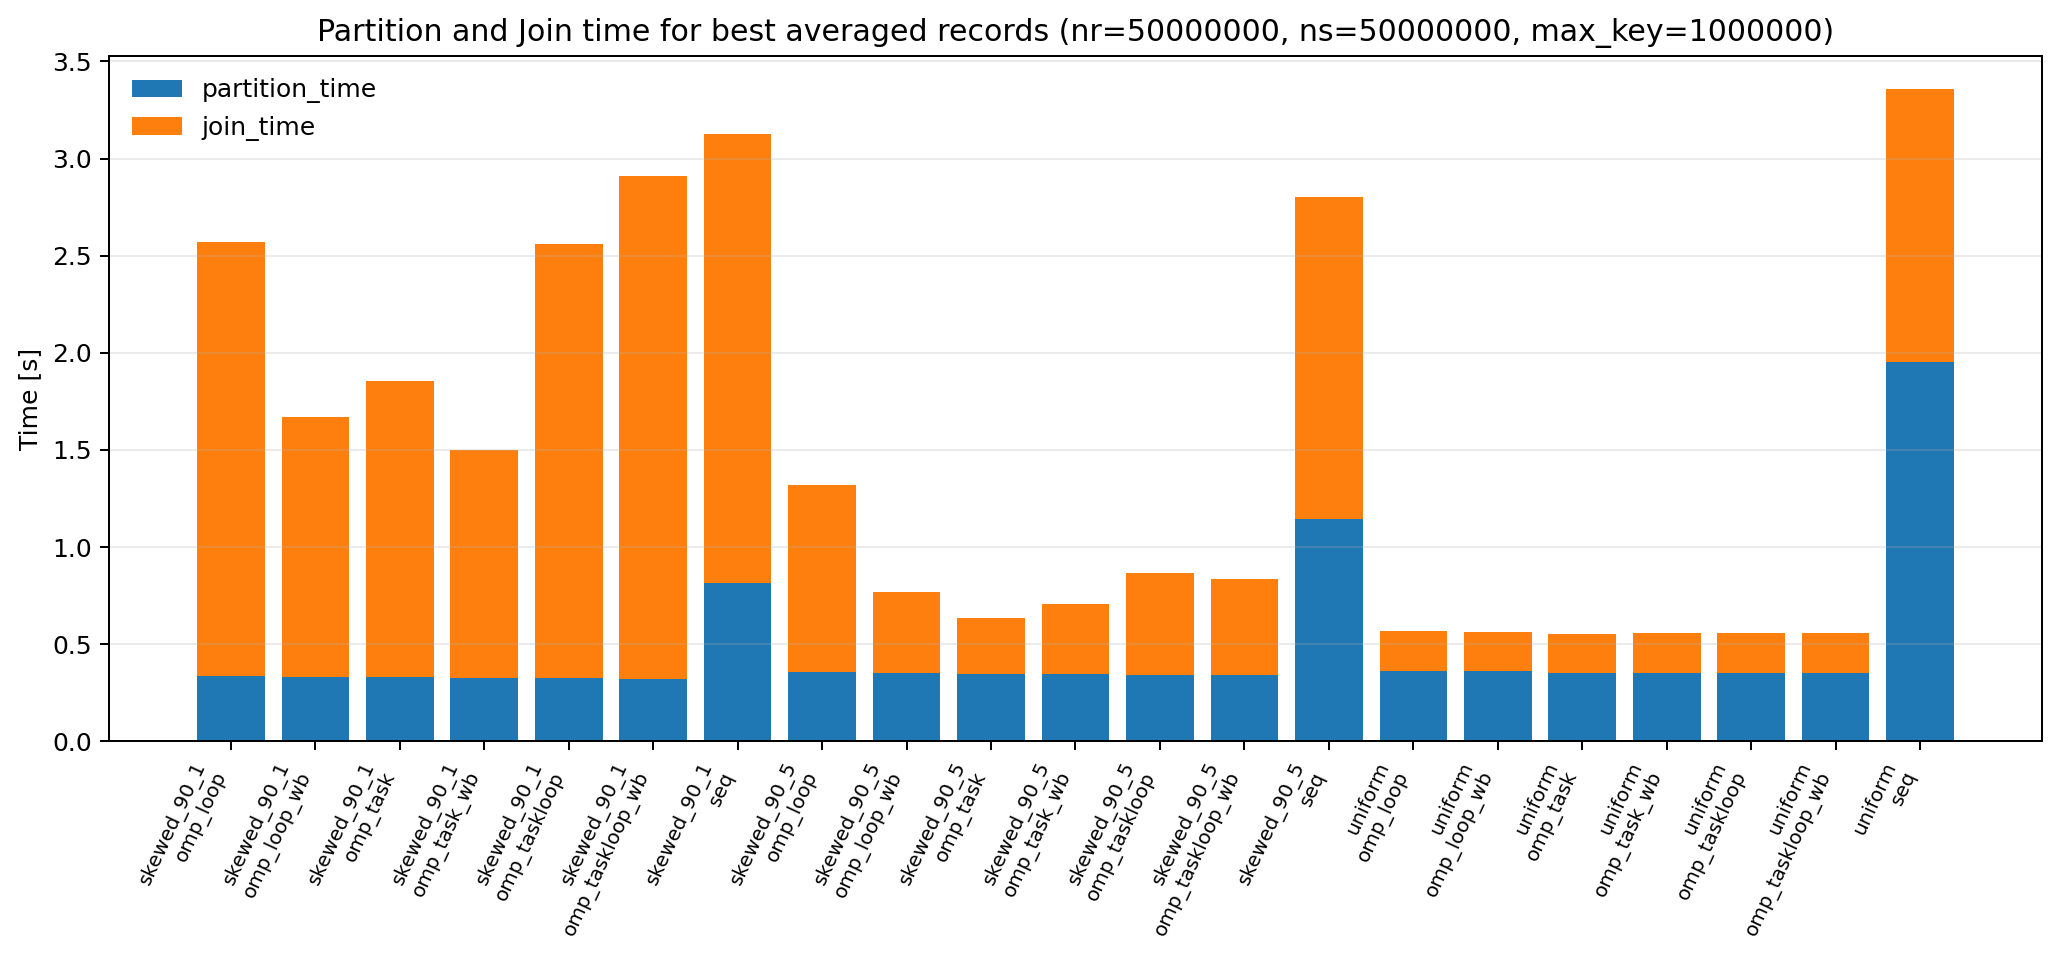
\includegraphics[width=0.82\linewidth]{../img/005_selected_best_phase_breakdown_50000000_50000000_1000000.png}
    \caption{Comparison between partition and join times for each dataset type and executables combination.}
    \label{fig:partition-join-time}
\end{figure}

The important distinction is between the non-\texttt{\_wb} and the \texttt{\_wb} executables. In the non-\texttt{\_wb} versions, the join work is submitted to OpenMP in the natural partition-id order \(0,\ldots,P-1\). This is simple and works well when the dataset is uniform, because partitions have similar sizes and each local join has roughly similar cost.
With skewed datasets, however, some partitions contain many more records and duplicate matches. Then a raw partition-id order can create a tail effect: most threads finish their small partitions while some few threads remain busy on hot partitions. The \texttt{\_wb} variants address this by keeping the same local hash-join logic, but changing the work list given to OpenMP. 
Before the join starts, the work of each partition is estimated as \(|R_p| + |S_p|\), and a target amount of records per join thread is computed. Partitions are sorted from largest to smallest and large partitions are assigned more than one logical thread by splitting their \(S_p\) probe range into subranges. Each subrange builds a private count table over the corresponding \(R_p\) partition, probes only its assigned part of \(S_p\), and writes into a private result slot; therefore no mutex is needed in the join hot path.


% Results Analysis
\section{Results Analysis}
All results below can be found in the \texttt{statistics.ipynb} notebook whose analyzed data are picked from \texttt{src/results/*.csv}. The best Module 2 C++ threaded result was \(0.507\) s for \texttt{hashjoin\_par\_pj\_wb\_map}; the best averaged OpenMP result in the final campaign is \(0.553\) s, so the final OpenMP implementation is close in absolute time but does not clearly improve over the previous C++ threaded best case. This section covers the main Module 3 comparison: sequential baseline, OpenMP loop, OpenMP tasks, the extra taskloop experiment, uniform/skewed workloads, and the previous C++ threaded implementation.

\begin{figure}[H]
    \centering
    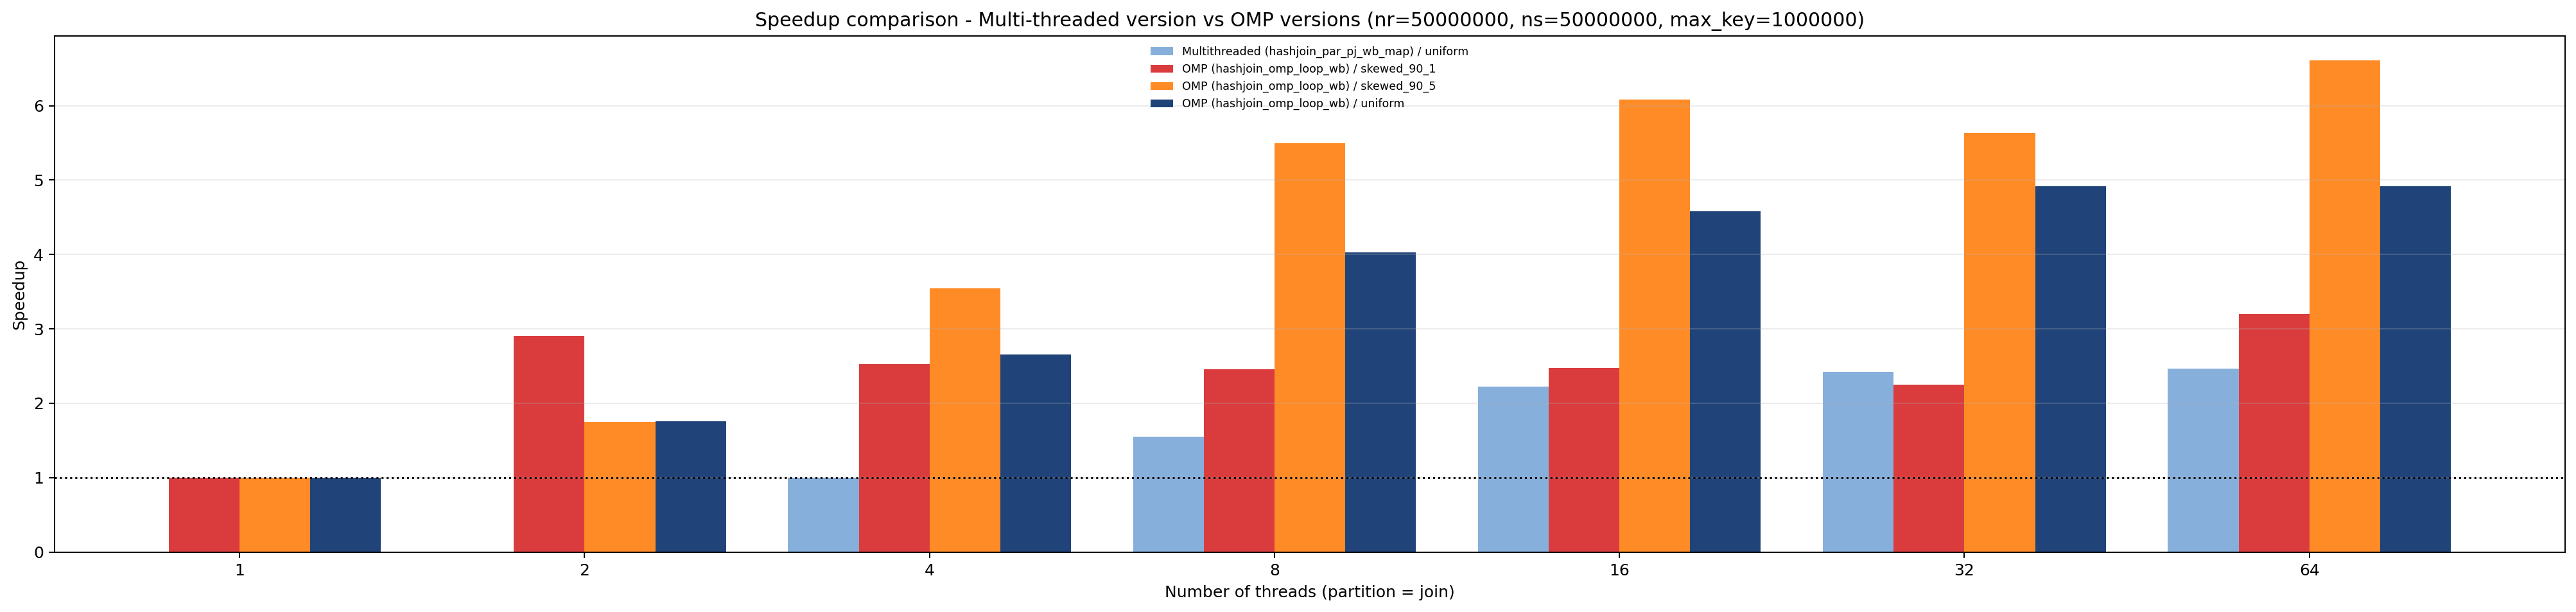
\includegraphics[width=0.90\linewidth]{../img/007_strong_scaling_speedup_50000000_50000000_1000000.png}
    \caption{Speedup comparison between the previous multi-threaded \texttt{hashjoin\_par\_pj\_wb\_map} executable and the selected OpenMP workload-balanced loop implementation.}
    \label{fig:module2-vs-omp-speedup}
\end{figure}


% Uniform dataset
\subsection{Uniform dataset}
On the uniform workload, all complete OpenMP implementations are close once both partition and join are parallelized. The best averaged time is obtained by \texttt{hashjoin\_omp\_task} with 64 partition threads and 32 join threads: \(0.553\) s, corresponding to \(6.08\times\) speedup over the current sequential baseline.

The difference between the best loop, task and taskloop versions is small; this means that, for uniform partitions, OpenMP tasking does not add much by itself. The dominant gains come from parallelizing the join and from keeping the local hash table cache-friendly.
Inside the required implementations, explicit tasks are slightly faster than loop scheduling on uniform data: \texttt{omp\_task} reaches \(0.553\) s against \(0.571\) s for \texttt{omp\_loop}. The extra taskloop variant remains very close to the best result and is also simpler to express than manual task creation, because OpenMP handles the task generation from the loop structure.

\begin{table}[H]
    \centering
    \small
    \begin{tabular}{lrrrr}
        \toprule
        Variant & \(T_{part}\) & \(T_{join}\) & Best time [s] & Speedup \\
        \midrule
        \texttt{omp\_loop} & 32 & 32 & 0.5714 & \(5.89\times\) \\
        \texttt{omp\_loop\_wb} & 32 & 32 & 0.5670 & \(5.93\times\) \\
        \texttt{omp\_task} & 64 & 32 & 0.5533 & \(6.08\times\) \\
        \texttt{omp\_task\_wb} & 64 & 32 & 0.5580 & \(6.03\times\) \\
        \texttt{omp\_taskloop} & 64 & 32 & 0.5576 & \(6.03\times\) \\
        \texttt{omp\_taskloop\_wb} & 64 & 32 & 0.5579 & \(6.03\times\) \\
        \bottomrule
    \end{tabular}
    \caption{Best averaged uniform-dataset configuration per OpenMP executable.}
    \label{tab:uniform-best}
\end{table}

\begin{figure}[H]
    \centering
    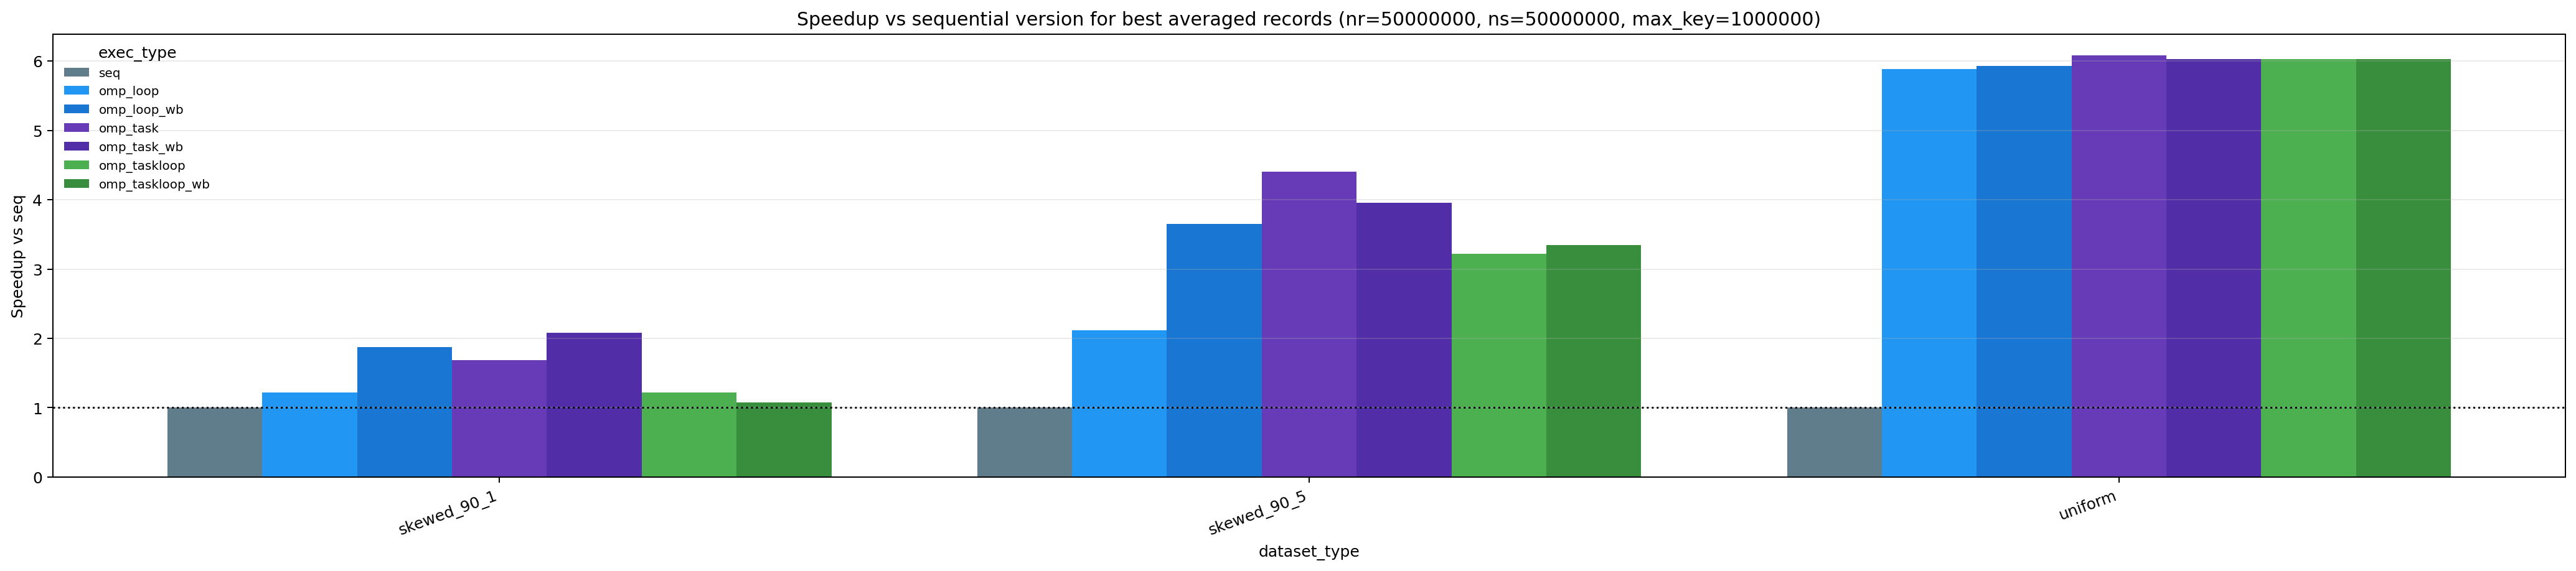
\includegraphics[width=0.82\linewidth]{../img/004_selected_best_Speedup_vs_Sequential_version_50000000_50000000_1000000.png}
    \caption{Best speedup against the sequential baseline for the current OpenMP campaign.}
    \label{fig:selected-best}
\end{figure}


% Skewed datasets
\subsection{Skewed datasets}
The skewed datasets change both load balance and the actual join workload. In the skewed runs, the final match count rises from about \(2.50 \cdot 10^9\) on uniform data to \(4.06 \cdot 10^{10}\) on \texttt{skewed\_90\_5} and \(1.74 \cdot 10^{11}\) on \texttt{skewed\_90\_1}.
This happens because many records are concentrated into a small set of hot partitions and hot keys, increasing the probability that the same keys appear many times in both relations.
Therefore the slowdown is not only scheduling overhead: the hot partitions also contain many more duplicate-key matches.

\begin{table}[H]
    \centering
    \scriptsize
    \begin{tabular}{llrrrrr}
        \toprule
        Dataset & Variant & \(T_{part}\) & \(T_{join}\) & Best time [s] & Join time [s] & Speedup \\
        \midrule
        \texttt{skewed\_90\_5} & \texttt{omp\_loop} & 32 & 32 & 1.3231 & 0.9660 & \(2.12\times\) \\
        \texttt{skewed\_90\_5} & \texttt{omp\_loop\_wb} & 32 & 32 & 0.7687 & 0.4131 & \(3.65\times\) \\
        \texttt{skewed\_90\_5} & \texttt{omp\_task} & 64 & 32 & 0.6365 & 0.2862 & \(4.41\times\) \\
        \texttt{skewed\_90\_5} & \texttt{omp\_task\_wb} & 64 & 32 & 0.7096 & 0.3617 & \(3.95\times\) \\
        \texttt{skewed\_90\_5} & \texttt{omp\_taskloop} & 64 & 32 & 0.8715 & 0.5267 & \(3.22\times\) \\
        \texttt{skewed\_90\_5} & \texttt{omp\_taskloop\_wb} & 64 & 32 & 0.8392 & 0.4971 & \(3.34\times\) \\
        \midrule
        \texttt{skewed\_90\_1} & \texttt{omp\_loop} & 32 & 32 & 2.5730 & 2.2363 & \(1.22\times\) \\
        \texttt{skewed\_90\_1} & \texttt{omp\_loop\_wb} & 32 & 32 & 1.6700 & 1.3342 & \(1.87\times\) \\
        \texttt{skewed\_90\_1} & \texttt{omp\_task} & 64 & 32 & 1.8562 & 1.5210 & \(1.69\times\) \\
        \texttt{skewed\_90\_1} & \texttt{omp\_task\_wb} & 64 & 32 & 1.5009 & 1.1705 & \(2.08\times\) \\
        \texttt{skewed\_90\_1} & \texttt{omp\_taskloop} & 64 & 32 & 2.5613 & 2.2338 & \(1.22\times\) \\
        \texttt{skewed\_90\_1} & \texttt{omp\_taskloop\_wb} & 64 & 32 & 2.9116 & 2.5861 & \(1.07\times\) \\
        \bottomrule
    \end{tabular}
    \caption{Best averaged skewed-dataset result for each OpenMP executable, using the sequential row with the same dataset label as baseline.}
    \label{tab:skewed-best}
\end{table}

The workload-balanced loop version has the largest improvement with skewness from non-\texttt{\_wb} to \texttt{\_wb}, but is still slower than the task \texttt{\_wb} version. For \texttt{skewed\_90\_5}, the loop version improves from \(1.323\) s to \(0.769\) s when workload balancing is enabled. For \texttt{skewed\_90\_1}, the same change improves from \(2.573\) s to \(1.670\) s. The strongest skew still remains slower because splitting the probe side of a hot partition helps load balance but also repeats the \(R_p\) build work for each subrange.

Explicit tasks give the best required result on both skewed datasets in the current averaged campaign: \texttt{omp\_task} reaches \(0.636\) s on \texttt{skewed\_90\_5}, while \texttt{omp\_task\_wb} reaches \(1.501\) s on \texttt{skewed\_90\_1}.
The extra taskloop implementation remains useful experimentally, but its workload-balanced version is mixed in these runs with a high speedup on \texttt{skewed\_90\_5} but very low one on \texttt{skewed\_90\_1}.


% Scaling analysis
\section{Scaling analysis}
Strong and weak scalability are measured only with the selected workload-balanced loop implementation, using the best fixed parameters found in the reduced grid. The loop version is used because it has the more balanced and expected behavior.

Both scaling files fix \(P=256\), \texttt{seed=13}, \texttt{max\_key=1\,000\,000}, guided partition and join schedules, partition/join chunk size \(8\), and partition block size \(32768\). In \texttt{strong\_scaling.cpp}, \(N_R=N_S=50\,000\,000\) is also fixed, while the only non-fixed parameter is the thread count, using the same value for partition and join phases. In \texttt{weak\_scaling.cpp}, both \(N_R=N_S\) and the thread count vary together, again with the same thread count for partition and join phases; their concrete values are reported in the plots below.


% Weak scalability
\subsection{Weak scalability}
Weak scaling worsens as the skew becomes stronger. On uniform data, increasing \(N\) together with the number of threads is still useful: the scaled speedup reaches about \(3.17\times\) at 16 threads and remains close to \(3.02\times\) at 32 threads. With moderate skew, \texttt{skewed\_90\_5}, the curve is lower and peaks earlier, at about \(2.36\times\) with 8 threads, then stays near \(2.1\times\) at 16 and 32 threads. With the strongest skew, \texttt{skewed\_90\_1}, the 2-thread case is almost ideal, but the curve then decreases to about \(1.30\times\) at 32 threads, because increasing \(N\) also increases the hot partitions and duplicate-key work that cannot be spread as evenly.

% Strong scalability
\subsection{Strong scalability}
Strong scaling shows a different effect of skew because the input size is fixed and the baseline is the 1-thread execution of each dataset. Uniform data improves regularly up to about \(4.92\times\) at 32 threads and then saturates at 64 threads. The moderate-skew case, \texttt{skewed\_90\_5}, has a slower 1-thread baseline and still contains enough work to split across threads, so its relative speedup is higher, reaching about \(6.48\times\) at 64 threads. The strongest skew, \texttt{skewed\_90\_1}, is not monotonic: it reaches about \(3.13\times\) at 2 threads, then stays below \(3\times\) for the larger thread counts. This shows that, when only a few hot partitions dominate the join, adding threads gives limited benefit even with workload balancing.

\begin{figure}[H]
    \centering
    \begin{minipage}[t]{0.45\linewidth}
        \centering
        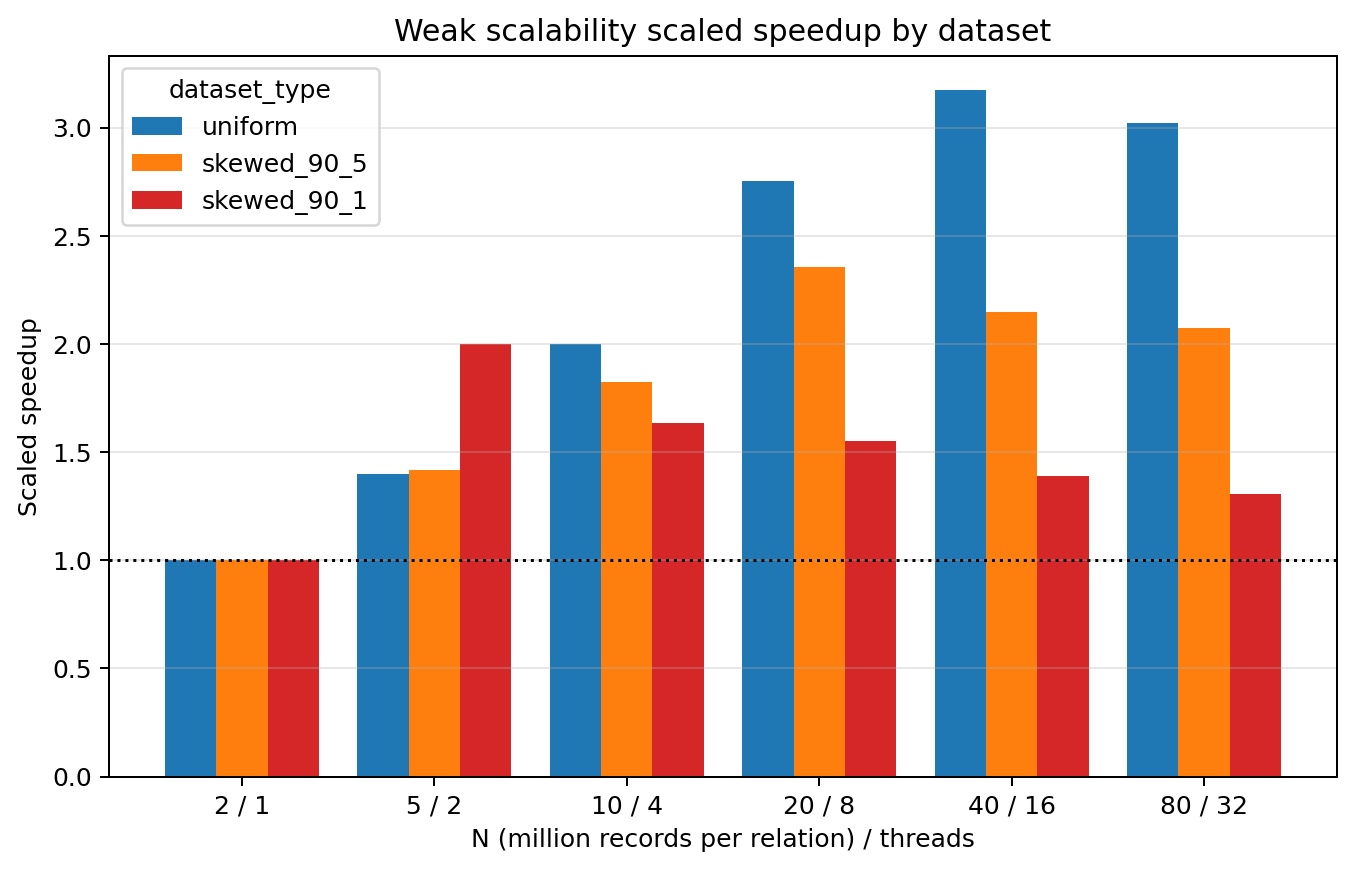
\includegraphics[width=\linewidth]{../img/013_weak_scalability_scaled_speedup_by_dataset.png}
        \caption{Weak-scaling scaled speedup for uniform and skewed datasets.}
        \label{fig:weak-scaling}
    \end{minipage}
    \hfill
    \begin{minipage}[t]{0.45\linewidth}
        \centering
        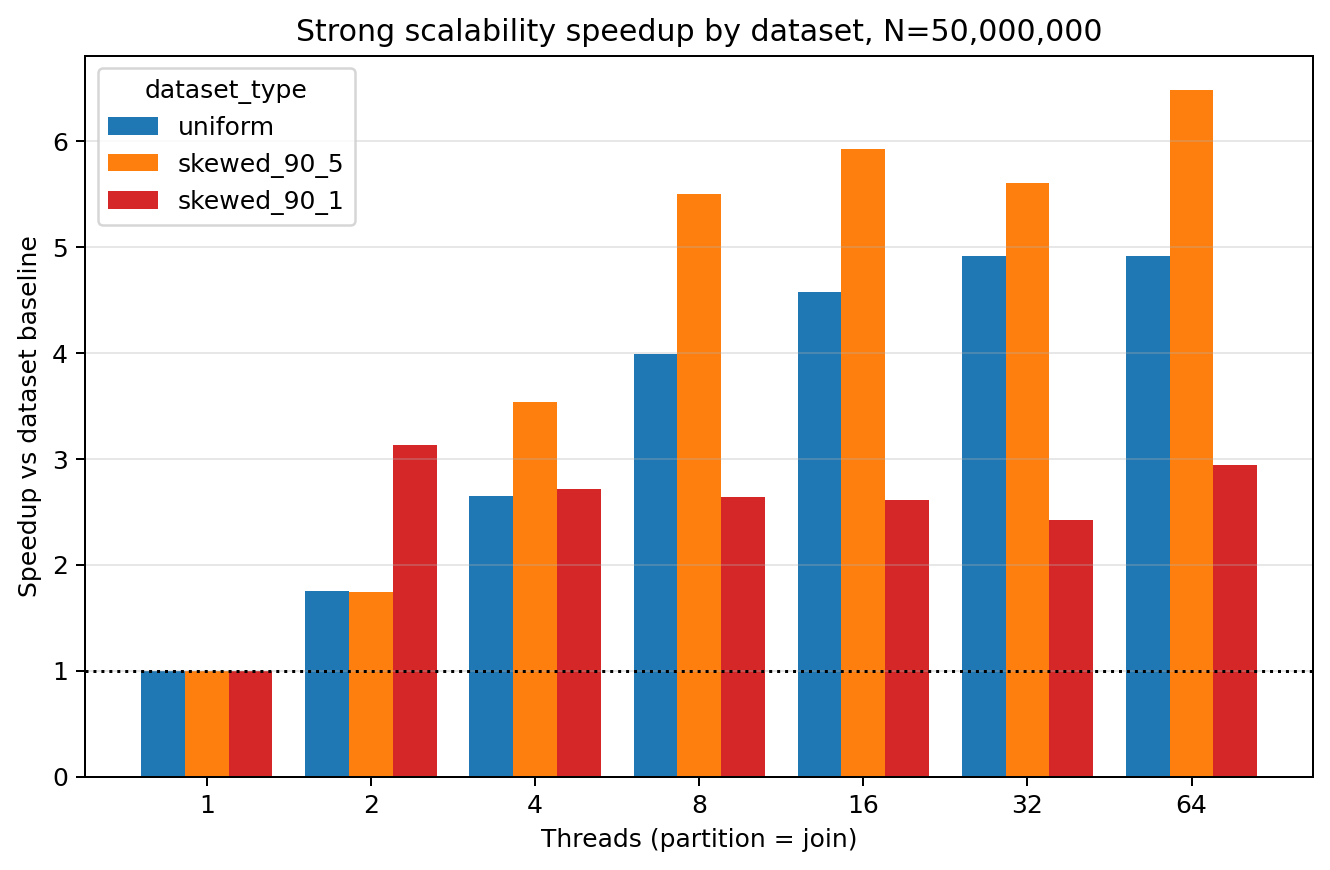
\includegraphics[width=\linewidth]{../img/011_strong_scalability_speedup_by_dataset.png}
        \caption{Strong-scaling speedup for the dedicated workload-balanced OpenMP executable.}
        \label{fig:strong-scaling}
    \end{minipage}
\end{figure}


% Correctness validation
\section{Correctness Validation}
Correctness is checked at two levels. For small inputs, \(N_R \leq 500\) and \(N_S \leq 500\), each executable runs the naive \(O(N_RN_S)\) verifier and compares its \texttt{join\_count}, \texttt{checksum1} and \texttt{checksum2} with the optimized result. If the comparison succeeds, the executable prints and records \texttt{verified=true}; if it fails, it prints \texttt{verified=false} and exits with an error. The checker therefore treats \texttt{verified=true} outputs as already validated by the exact naive oracle.

For benchmark-size inputs, where the naive verifier is too expensive, \texttt{checker.cpp} scans the Slurm output files and compares \texttt{join\_count}, \texttt{checksum1} and \texttt{checksum2} within each executable and dataset-type group. This checks that repeated runs of the same configuration family are deterministic and mutually consistent; it is not a cross-executable reference checker.

% Conclusions
\section{Conclusions}
The OpenMP implementations preserve the previous algorithm and make the scheduling tradeoffs clearer. On uniform data, loop, task and taskloop variants perform similarly once the join phase is parallelized; tasking does not provide a large advantage because partitions are already well balanced. On skewed data, workload-aware join decomposition is the decisive change for the loop family, while explicit tasks give the best required results in the current averaged campaign. The strongest skew still exposes a limitation: splitting a hot partition's probe range improves balance, but the repeated private build phase can become expensive.

The scalability results confirm the same trend: uniform data scales more regularly, moderate skew can still exploit extra threads, while the strongest skew quickly becomes limited by hot partitions and duplicate-key work.

Compared with the best C++ threaded result from Module 2, the best OpenMP result is close but slightly slower in the final campaign. The main benefit of this module is therefore not a new absolute minimum, but a clearer understanding of which OpenMP constructs are sufficient and how join-work decomposition affects uniform and skewed workloads.

\end{document}
